\documentclass[12pt]{article}
\usepackage{cwilliams-standard}

\setclass{\MLONE}
\settitle{Machine Learning 1 - Homework 4}

\begin{document}

\maketitlepage

\section{Phase 1}

\subsection{Two Classes}

\subsubsection{Scatter Plot}


\begin{figure}[H]
\centering
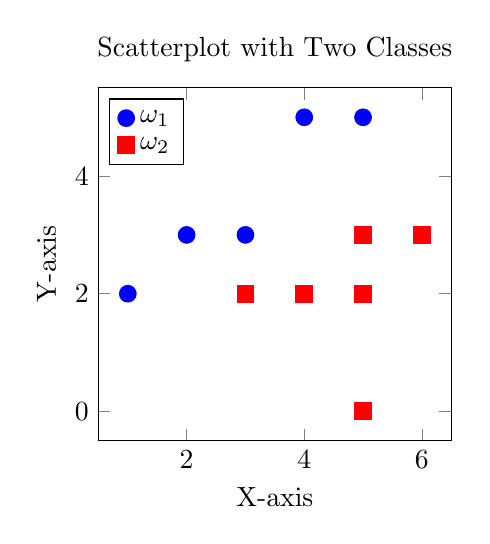
\begin{tikzpicture}
\begin{axis}[
    width=0.5\textwidth,
    height=0.5\textwidth,
    xlabel={X-axis},
    ylabel={Y-axis},
    title={Scatterplot with Two Classes},
    legend pos=north west
]

% Class 1
\addplot[
    only marks,
    mark=*,
    color=blue,
    mark size=3pt
] coordinates {
    (1, 2)
    (2, 3)
    (3, 3)
    (4, 5)
    (5, 5)
};

% Class 2
\addplot[
    only marks,
    mark=square*,
    color=red,
    mark size=3pt
] coordinates {
    (4, 2)
    (5, 0)
    (5, 2)
    (3, 2)
    (5, 3)
    (6, 3)
};

\legend{$\omega_1$, $\omega_2$}
\end{axis}
\end{tikzpicture}
\end{figure}


\vspace{-0.5cm}

\subsubsection{Class Variance}

To calculate the between-class variance, $S_B$, and the within-class indicator, $S_W$, we need to calculate the mean of each class, and the total mean.

\begin{align}
    \mu_1 = \frac{1}{n_1}\sum_{i=1}^{n_1} x_i^{(1)} &= \frac{1}{5} 
    \begin{bmatrix}
        1 + 2 + 3 + 4 + 5 \\
        2 + 3 + 3 + 5 + 5
    \end{bmatrix} = \frac{1}{5}
    \begin{bmatrix}
        15 \\
        18
    \end{bmatrix} = 
    \begin{bmatrix}
        3 \\
        3.6
    \end{bmatrix} \\
    \mu_2 = \frac{1}{n_2} \sum_{i=1}^{n_2} x_i^{(2)} &= \frac{1}{6} 
    \begin{bmatrix}
        4 + 5+ 5 + 3 +5 + 6 \\
        2 + 0 + 2 + 2 + 3 + 3
    \end{bmatrix} = 
    \frac{1}{6}
    \begin{bmatrix}
        28 \\
        12
    \end{bmatrix} =
    \begin{bmatrix}
        4.67 \\
        2
    \end{bmatrix} \\
    \mu_{tot} = \frac{1}{n_{tot}} \sum_{i=1}^{n_1+n_2} x_i^{(1 \& 2)} &= \frac{1}{11}
    \begin{bmatrix}
         1 + 2 + 3 + 4 + 5 + 4 + 5+ 5 + 3 +5 + 6 \\
         2 + 3 + 3 + 5 + 5 + 2 + 0 + 2 + 2 + 3 + 3
    \end{bmatrix} = 
    \frac{1}{11} 
    \begin{bmatrix}
        43 \\
        30
    \end{bmatrix} =
    \begin{bmatrix}
        3.91 \\
        2.73
    \end{bmatrix}
\end{align}

After finding the means, we can now find the between-class variance with this equation
\begin{equation}
    S_B = n_1 (\mu_1 - \mu_{tot})(\mu_1 - \mu)^T + n_2(\mu_2 - \mu_{tot})^T
\end{equation}

\begin{align}
    S_B = 5\Big( 
    \begin{bmatrix}
        3 - 3.91 \\
        3.6 - 2.73
    \end{bmatrix} 
    \begin{bmatrix}
        3 - 3.91 & 3.6 - 2.73
    \end{bmatrix}
    \Big)
    &+
    6 \Big( \begin
    {bmatrix}
        4.67 - 3.91 \\
        2 - 2.73
    \end{bmatrix} 
    \begin{bmatrix}
        4.67 - 3.91 & 2 - 2.73
    \end{bmatrix}
    \Big)
\end{align}
\begin{equation}
    \boxed{
    S_B =
    \begin{bmatrix}
        7.63 & -7.25 \\
        -7.25 & 6.98
    \end{bmatrix}
    }
\end{equation}

Next, we can find the within-class variance with this equation 

\begin{equation}
    S_W = \sum_{x_1 \in \omega_1} (x_1 - \mu_1)^T (x_1 - \mu_1) + \sum_{x_2 \in \omega_2} (x_2 - \mu_2)^T (x_2 - \mu_2)
\end{equation}

\begin{align}
    S_W = \begin{bmatrix}
        1 - 3 & 2 - 3.6 \\
        2 - 3 & 3 - 3.6 \\
        3 - 3 & 3 - 3.6 \\
        4 - 3 & 5 - 3.6 \\
        5 - 3 & 5 - 3.6
    \end{bmatrix}
    &\begin{bmatrix}
        1 -3 & 2 - 3 & 3 - 3 & 4 - 3 & 5 - 3 \\
        2 - 3.6 & 3 - 3.6 & 3 - 3.6 & 5 - 3.6 & 5 - 3.6
    \end{bmatrix}
    + \\
    \begin{bmatrix}
        4 - 4.6 & 2 - 2 \\
        5 - 4.6 & 0 - 2 \\
        5 - 4.6 & 2 - 2 \\
        3 - 4.6 & 2 - 2 \\
        5 - 4.6 & 3 - 2 \\
        6 - 4.6 & 3 - 2
    \end{bmatrix}
    &\begin{bmatrix}
        4 - 4.6 & 5 - 4.6 & 5 - 4.6 & 3 - 4.6 & 5 - 4.6 & 6 - 4.6 \\
        2 - 2 & 0 - 2 & 2 - 2 & 2 - 2 & 3 - 2 & 3 - 2
    \end{bmatrix} \\
    =
    \begin{bmatrix}
         10 & 8 \\
         8 & 7.2
    \end{bmatrix}
    &+
    \begin{bmatrix}
        5.33 & 1.00 \\
        1.00 & 6.00
    \end{bmatrix}
\end{align}

\begin{equation}
    S_W = 
    \boxed{
        \begin{bmatrix}
            15.33 & 9.00 \\
            9.00 & 13.20
        \end{bmatrix}
    }
\end{equation}

\subsection{Spectral Decomposition of Fisher Criterion}

\subsubsection{Eigenvectors}
To find the direction that maximizes class separation, we solve the generalized eigenvectors:
\begin{equation}
    S_B \mathbf{w} = \lambda S_W \mathbf{w}
\end{equation}

This is the equivalent to finding eigenvalues and eigenvectors of $S_W^{-1}S_B$.

First, $S_W^{-1}$:
\begin{equation}
    \det(S_W) = 15.33 \times 13.20 - 9.00 \times 9.00 = 121.36
\end{equation}

\begin{equation}
    S_W^{-1} = \frac{1}{121.36}
    \begin{bmatrix}
        13.20 & -9.00 \\
        -9.00 & 15.33
    \end{bmatrix}
    =
    \begin{bmatrix}
        0.1087 & -0.0741 \\
        -0.0741 & 0.1263
    \end{bmatrix}
\end{equation}

Then $S_W^{-1}S_B$:
\begin{equation}
    S_W^{-1}S_B = 
    \begin{bmatrix}
        0.1087 & -0.0741 \\
        -0.0741 & 0.1263
    \end{bmatrix}
    \begin{bmatrix}
        7.63 & -7.25 \\
        -7.25 & 6.98
    \end{bmatrix}
    =
    \begin{bmatrix}
        1.362 & -1.308 \\
        -1.480 & 1.421
    \end{bmatrix}
\end{equation}


Solving the characteristic equation $\det(S_W^{-1}S_B - \lambda I) = 0$:
\begin{align}
    \lambda^2 - 2.78\lambda &= 0 \\
    \lambda_1 &= 2.78 \\
    \lambda_2 &= 0
\end{align}

For $\lambda_1 = 2.78$, the eigenvector is:
\begin{equation}
    \mathbf{w}_1 = \begin{bmatrix} -0.68 \\ 0.73 \end{bmatrix}
\end{equation}

For $\lambda_2 = 0$, the eigenvector is:
\begin{equation}
    \mathbf{w}_2 = \begin{bmatrix} 0.69 \\ 0.72 \end{bmatrix}
\end{equation}

\begin{figure}[H]
\centering
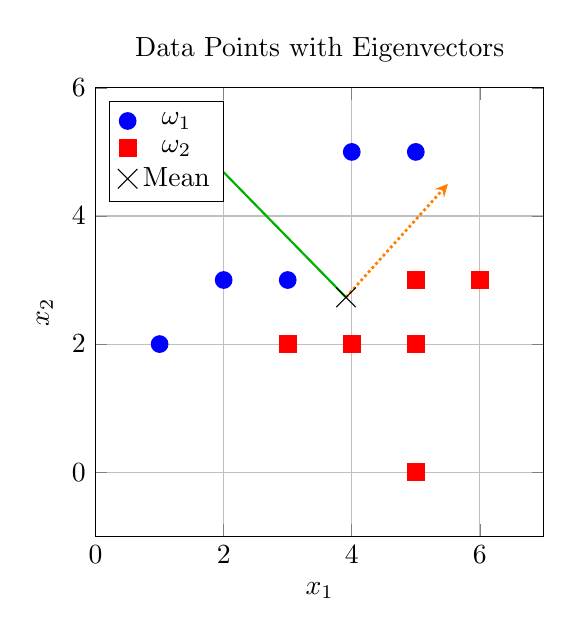
\begin{tikzpicture}
\begin{axis}[
    width=0.6\textwidth,
    height=0.6\textwidth,
    xlabel={$x_1$},
    ylabel={$x_2$},
    title={Data Points with Eigenvectors},
    legend pos=north west,
    xmin=0, xmax=7,
    ymin=-1, ymax=6,
    grid=major,
    axis equal image=false
]

% Class 1
\addplot[only marks, mark=*, color=blue, mark size=3pt] coordinates {
    (1, 2) (2, 3) (3, 3) (4, 5) (5, 5)
};

% Class 2
\addplot[only marks, mark=square*, color=red, mark size=3pt] coordinates {
    (4, 2) (5, 0) (5, 2) (3, 2) (5, 3) (6, 3)
};

% Overall mean
\addplot[only marks, mark=x, color=black, mark size=5pt] coordinates {(3.91, 2.73)};

% Eigenvector 1 (scaled for visibility)
\addplot[thick, color=green!70!black, -stealth] coordinates {(3.91, 2.73) (1.2, 5.5)};
% \node at (axis cs:0.5,5.8) {$\mathbf{w}_1$ ($\lambda=2.783$)};

% Eigenvector 2 (scaled for visibility, dotted and smaller)  
\addplot[densely dotted, color=orange, -stealth, line width=1pt] coordinates {(3.91, 2.73) (5.5, 4.5)};
% \node at (axis cs:6.8,5.8) {$\mathbf{w}_2$ ($\lambda=0$)};

\legend{$\omega_1$, $\omega_2$, Mean}
\end{axis}
\end{tikzpicture}
\caption{Eigenvectors plotted from the overall mean. $\mathbf{w}_1$ (green) corresponds to $\lambda_1 = 2.783$ and provides maximum class separation. $\mathbf{w}_2$ (orange, dotted) corresponds to $\lambda_2 = 0$ and provides no discriminative information.}
\end{figure}

\subsubsection{Display Data}

Projecting the data onto eigenvector $\mathbf{w}_1 = [-0.67, 0.73]^T$:

For each point $\mathbf{x}$, the projection is $y = \mathbf{w}_1^T \mathbf{x} = -0.67x_1 + 0.73x_2$.

\textbf{Class 1 projections:}
\begin{align*}
    (1,2): &\quad y = -0.67(1) + 0.73(2) = 0.79 \\
    (2,3): &\quad y = -0.67(2) + 0.73(3) = 0.85 \\
    (3,3): &\quad y = -0.67(3) + 0.73(3) = 0.17 \\
    (4,5): &\quad y = -0.67(4) + 0.73(5) = 0.97 \\
    (5,5): &\quad y = -0.67(5) + 0.73(5) = 0.29
\end{align*}
Mean: $\bar{y}_1 = 0.61$

\textbf{Class 2 projections:}
\begin{align*}
    (4,2): &\quad y = -0.67(4) + 0.73(2) = -1.23 \\
    (5,0): &\quad y = -0.67(5) + 0.73(0) = -3.38 \\
    (5,2): &\quad y = -0.67(5) + 0.73(2) = -1.91 \\
    (3,2): &\quad y = -0.67(3) + 0.73(2) = -0.55 \\
    (5,3): &\quad y = -0.67(5) + 0.73(3) = -1.17 \\
    (6,3): &\quad y = -0.67(6) + 0.73(3) = -1.85
\end{align*}
Mean: $\bar{y}_2 = -1.68$

\begin{figure}[H]
\centering
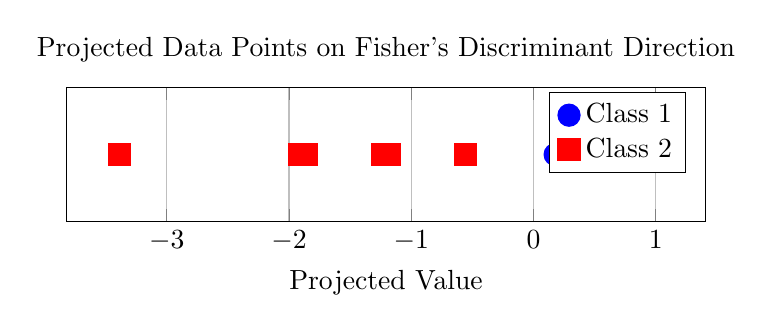
\begin{tikzpicture}
\begin{axis}[
    width=0.8\textwidth,
    height=0.27\textwidth,
    xlabel={Projected Value},
    title={Projected Data Points on Fisher's Discriminant Direction},
    ytick=\empty,
    ymin=-0.5, ymax=0.5,
    grid=major,
    legend pos=north east
]
% Class 1
\addplot[only marks, mark=*, color=blue, mark size=4pt] coordinates {
    (0.795, 0) (0.854, 0) (0.177, 0) (0.972, 0) (0.295, 0)
};
% Class 2
\addplot[only marks, mark=square*, color=red, mark size=4pt] coordinates {
    (-1.236, 0) (-3.385, 0) (-1.913, 0) (-0.559, 0) (-1.177, 0) (-1.854, 0)
};

% Optional: Add mean markers
% \addplot[only marks, mark=|, color=blue, mark size=10pt, line width=2pt] coordinates {(0.619, 0)};
% \addplot[only marks, mark=|, color=red, mark size=10pt, line width=2pt] coordinates {(-1.687, 0)};

\legend{Class 1, Class 2, Class 1 Mean, Class 2 Mean}
\end{axis}
\end{tikzpicture}
\caption{Projected data points showing clear separation between classes along the discriminant direction.}
\end{figure}

\subsection{Reduce Dimensionality}

\subsubsection{Plot of Probability Density}

\textbf{Choice of projection direction:} We choose eigenvector $\mathbf{w}_1 = [-0.67, 0.73]^T$ for the projection because it corresponds to the largest eigenvalue ($\lambda_1 = 2.783$), which maximizes the Fisher criterion. This direction maximizes the ratio of between-class variance to within-class variance, providing optimal class separation.

The second eigenvector $\mathbf{w}_2$ has eigenvalue $\lambda_2 = 0$, meaning it provides no discriminative information and would not help separate the classes.

After projection, Class 1 has mean 0.619 and Class 2 has mean -1.687, showing clear separation in the 1D subspace.

\subsection{L2 Distance Calculations}

\textbf{Before LDA (Original 2D space):}
\begin{equation}
    ||\mu_1 - \mu_2||_2 = \sqrt{(3 - 4.6)^2 + (3.6 - 2)^2} = \sqrt{2.77 + 2.56} = \sqrt{5.338} = 2.31
\end{equation}

\textbf{After LDA (Projected 1D space):}
\begin{equation}
    |\bar{y}_1 - \bar{y}_2| = |0.61 - (-1.68)| = |2.30| = 2.30
\end{equation}

\textbf{Comparison:}
\begin{itemize}
    \item Distance before LDA: 2.31
    \item Distance after LDA: 2.30
    \item Difference: 0.01 (0.22\%)
\end{itemize}

The L2 distance between class means is nearly preserved after projection (difference of only 0.005). This demonstrates that Fisher's LDA successfully identifies the projection direction that maintains class separation while reducing dimensionality from 2D to 1D. The small reduction is expected and shows that the discriminant direction $\mathbf{w}_1$ captures almost all the information relevant for class separation.

% \begin{figure}[H]
% \centering
% \begin{tikzpicture}
% \begin{axis}[
%     width=0.5\textwidth,
%     height=0.5\textwidth,
%     xlabel={Projected Value},
%     ylabel={Density},
%     title={Probability Density Functions of Projected Data},
%     legend pos=north west,
%     ymin=0,
%     ymax=0.6,
%     grid=major
% ]

% % Class 1 - Approximate PDF (using histogram bins)
% \addplot[
%     ybar interval,
%     fill=blue,
%     fill opacity=0.3,
%     draw=blue,
%     line width=1.5pt
% ] coordinates {
%     (0.1, 0.4)
%     (0.3, 0.5)
%     (0.5, 0.4)
%     (0.7, 0.5)
%     (0.9, 0.5)
%     (1.1, 0.3)
% };

% % Class 2 - Approximate PDF
% \addplot[
%     ybar interval,
%     fill=red,
%     fill opacity=0.3,
%     draw=red,
%     line width=1.5pt
% ] coordinates {
%     (-3.5, 0.2)
%     (-3.0, 0.3)
%     (-2.5, 0.2)
%     (-2.0, 0.35)
%     (-1.5, 0.4)
%     (-1.0, 0.35)
%     (-0.5, 0.2)
%     (0.0, 0.1)
% };

% \legend{Class 1, Class 2}
% \end{axis}
% \end{tikzpicture}
% \end{figure}

\begin{figure}[H]
    \centering
    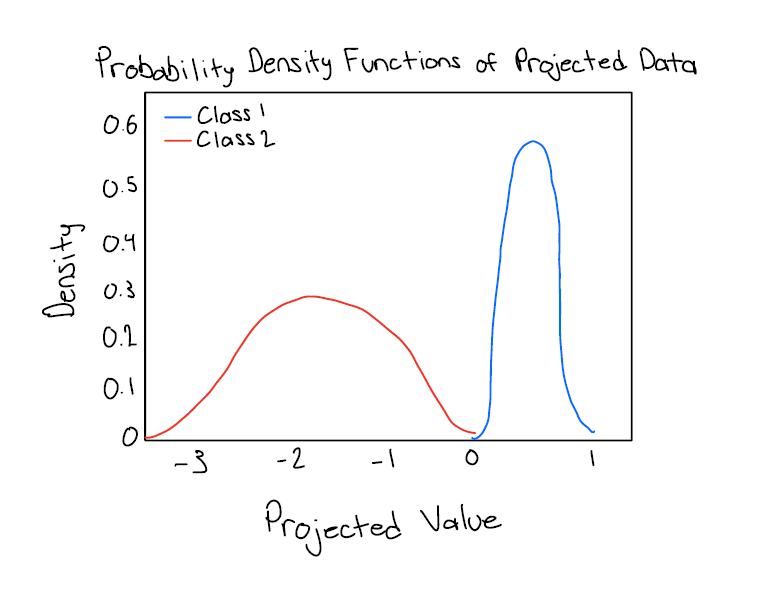
\includegraphics[width=0.75\linewidth]{images/sketch_of_proability_density_function.png}
    \caption{Sketch of Probabiltiy Dense Function}
    \label{fig:probabilitysketch}
\end{figure}

\newpage
\section{Phase 2}

\subsection{Politician Face's Dataset} \label{sec:politiciansfaces}

The number of unique politicians (classes) are in the dataset is \boxed{82}.

The number of observations (images) in the dataset is \boxed{3382}

The dimensionality of the dataset is \boxed{2914}

The names of all the politicians in this dataset are as follows:
\begin{multicols}{3}
\begin{enumerate}[itemsep=0pt]
    \item Abdullah Gul
    \item Alejandro Toledo
    \item Alvaro Uribe
    \item Amelie Mauresmo
    \item Andre Agassi
    \item Angelina Jolie
    \item Ariel Sharon
    \item Arnold Schwarzenegger
    \item Atal Bihari Vajpayee
    \item Bill Clinton
    \item Bill Gates
    \item Carlos Menem
    \item Carlos Moya
    \item Colin Powell
    \item David Beckham
    \item Donald Rumsfeld
    \item Fidel Castro
    \item George Robertson
    \item George W Bush
    \item Gerhard Schroeder
    \item Gloria Macapagal Arroyo
    \item Gray Davis
    \item Guillermo Coria
    \item Hamid Karzai
    \item Hans Blix
    \item Hugo Chavez
    \item Igor Ivanov
    \item Jack Straw
    \item Jacques Chirac
    \item Jean Charest
    \item Jean Chretien
    \item Jennifer Aniston
    \item Jennifer Capriati
    \item Jennifer Lopez
    \item Jeremy Greenstock
    \item Jiang Zemin
    \item John Ashcroft
    \item John Bolton
    \item John Howard
    \item John Kerry
    \item John Negroponte
    \item John Snow
    \item Joschka Fischer
    \item Jose Maria Aznar
    \item Juan Carlos Ferrero
    \item Julianne Moore
    \item Junichiro Koizumi
    \item Kofi Annan
    \item Lance Armstrong
    \item Laura Bush
    \item Lindsay Davenport
    \item Lleyton Hewitt
    \item Luiz Inacio Lula da Silva
    \item Mahmoud Abbas
    \item Megawati Sukarnoputri
    \item Michael Bloomberg
    \item Michael Schumacher
    \item Naomi Watts
    \item Nestor Kirchner
    \item Nicole Kidman
    \item Paul Bremer
    \item Pervez Musharraf
    \item Pete Sampras
    \item Recep Tayyip Erdogan
    \item Renee Zellweger
    \item Ricardo Lagos
    \item Richard Myers
    \item Roh Moo-hyun
    \item Rudolph Giuliani
    \item Saddam Hussein
    \item Serena Williams
    \item Silvio Berlusconi
    \item Spencer Abraham
    \item Tiger Woods
    \item Tim Henman
    \item Tom Daschle
    \item Tom Ridge
    \item Tony Blair
    \item Venus Williams
    \item Vicente Fox
    \item Vladimir Putin
    \item Winona Ryder
\end{enumerate}
\end{multicols}

\subsection{First Twenty Politicians}
Here is the subplot containing the images of the first 20 politicians.

\begin{figure}[H]
    \centering
    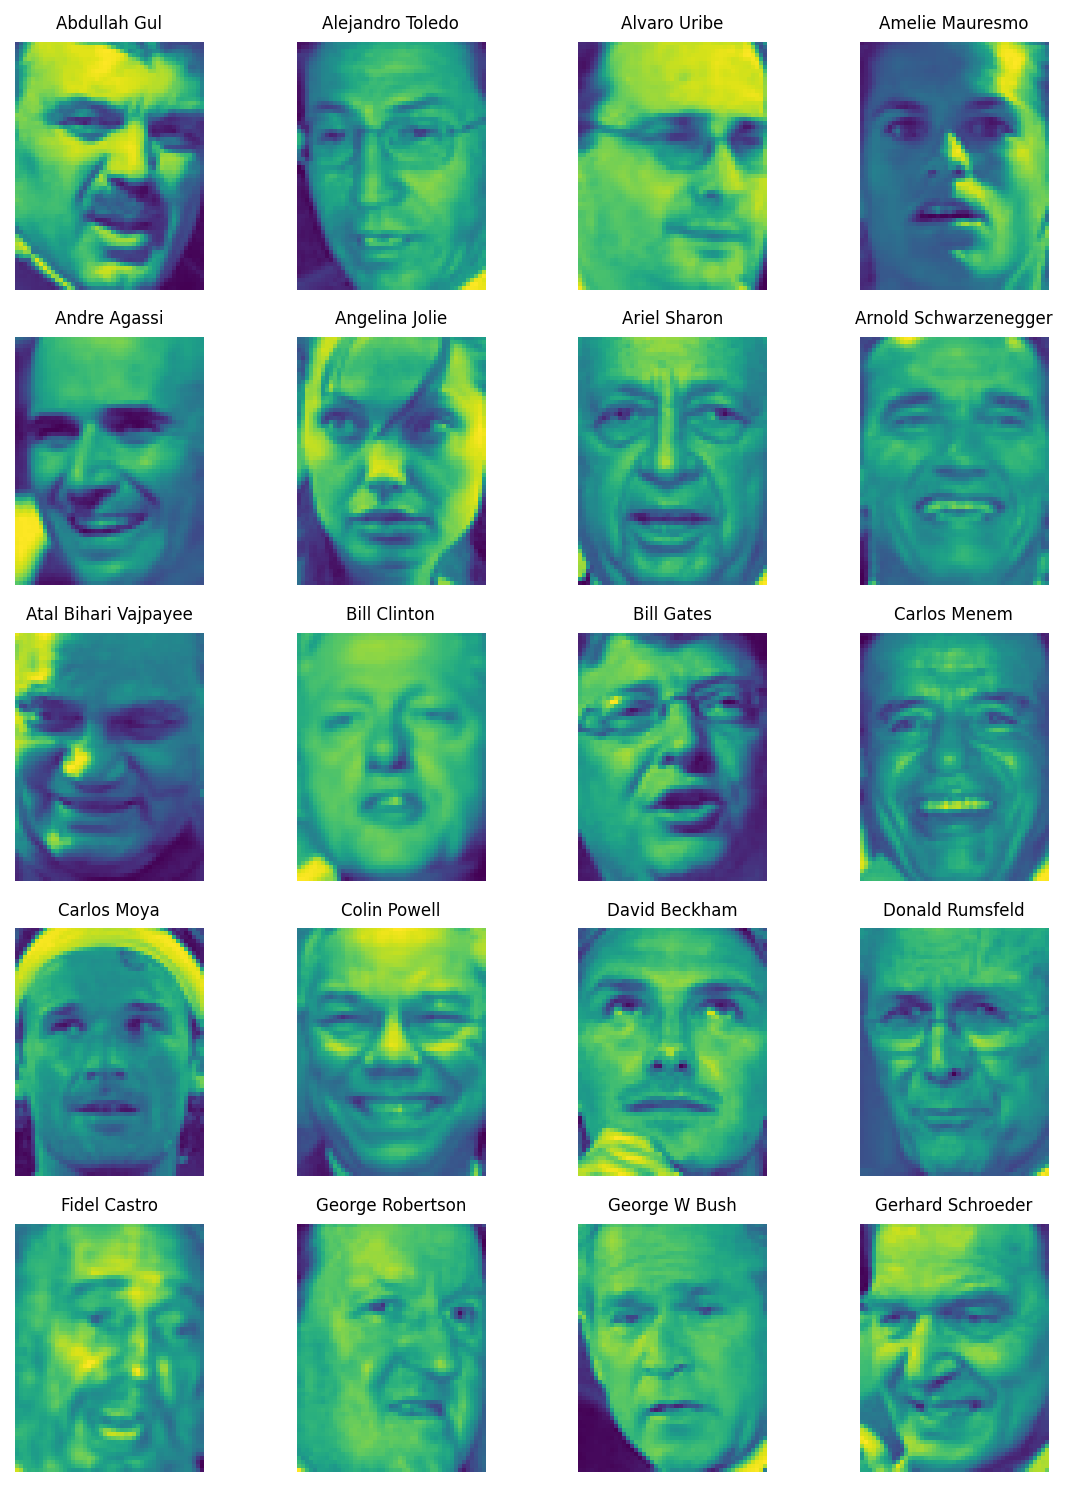
\includegraphics[width=0.75\linewidth]{images/first_20_politicians.png}
    \caption{Scatterplot of x vs. y with Eigenvectors}
    \label{fig:scatterplot}
\end{figure}

\subsection{Image Classification}

\subsubsection{Required Classes}

As determined in Question 5 (Section 2.1), it would be equal to the number of unique politicians in the dataset, which is 
\boxed{82}.

\subsubsection{Balanced Dataset?}

The dataset is very unbalanced. The minimum number of images per politician is 17, but the maximum for one politician is 530. These numbers are very unbalanced.

Here is a plot show casing the disparity.

\begin{figure}[H]
    \centering
    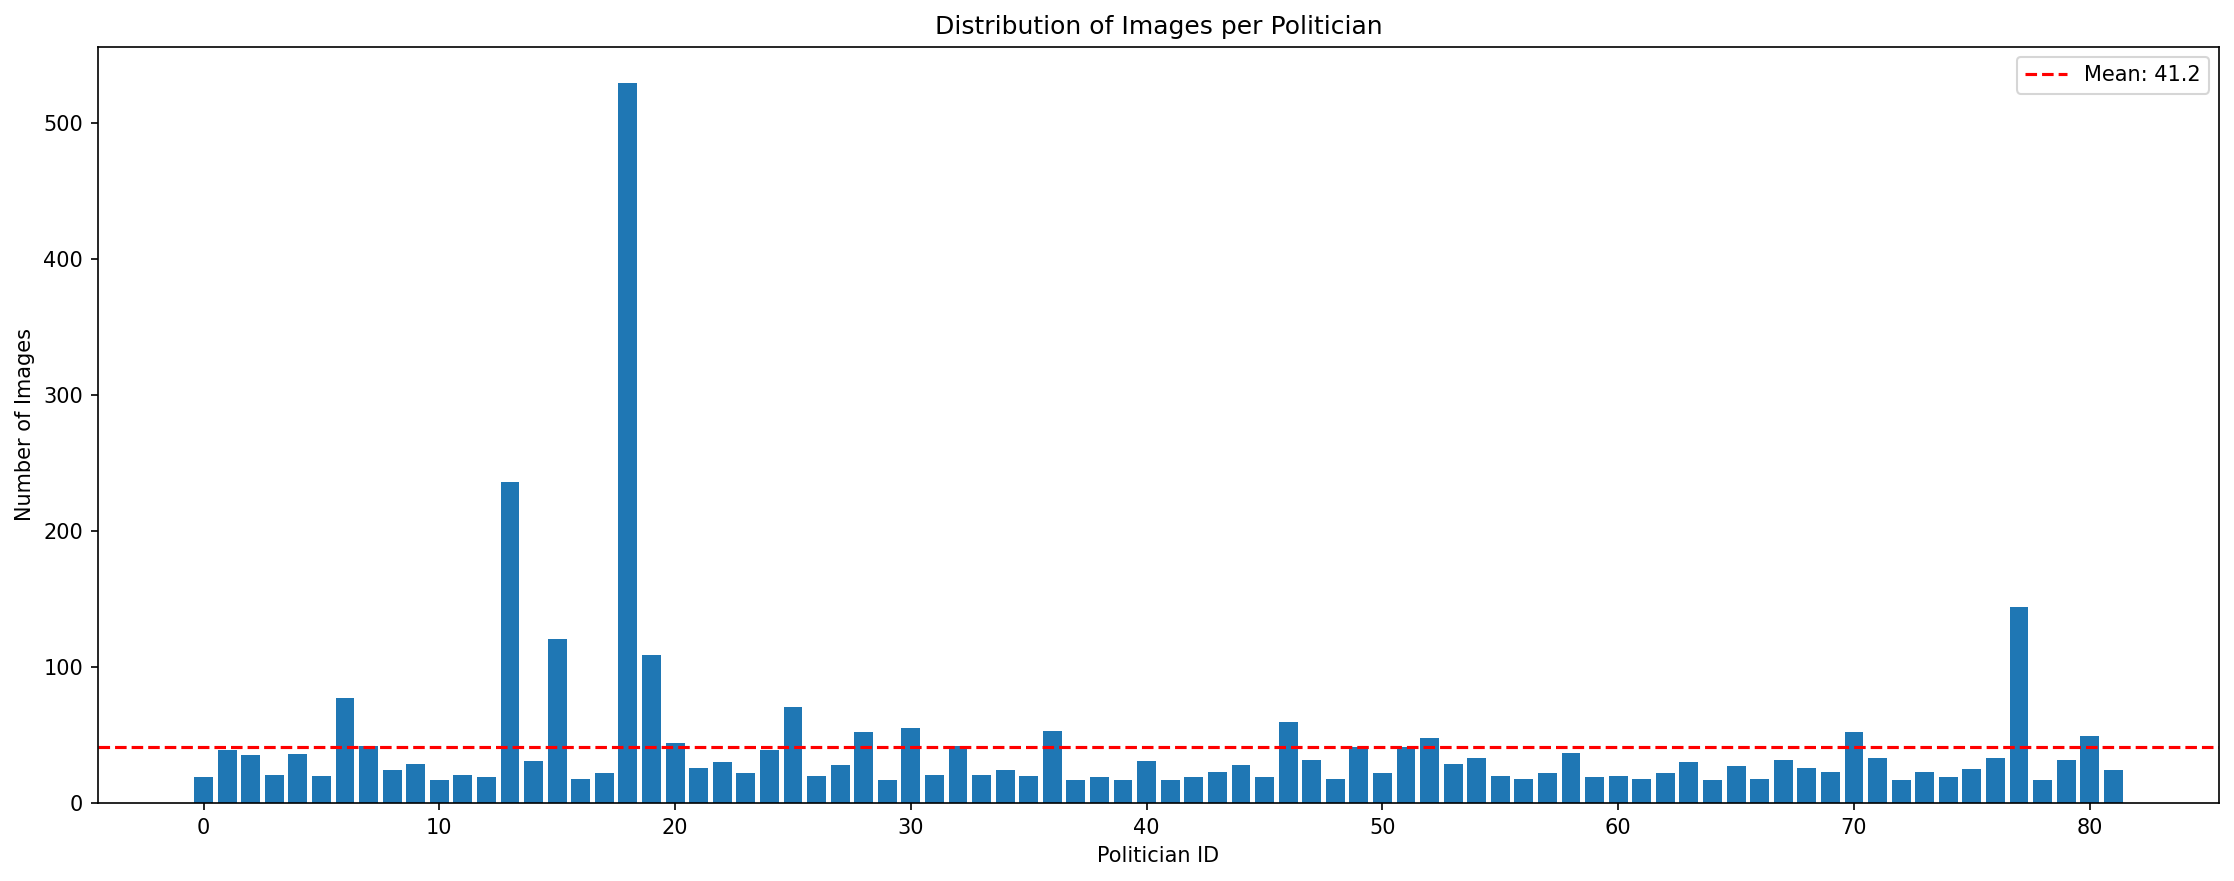
\includegraphics[width=0.8\linewidth]{images/distribution_of_politicians.png}
    \caption{Distribution of Images per Politician}
    \label{fig:distriplot}
\end{figure}

\subsection{Standardize and LDA}

Before computing the $S_B$ and $S_W$, we must standardize the data matrix 

\begin{lstlisting}
X_mean = X.mean(axis=0)  # mean of each feature
X_std = np.sqrt(((X - X_mean) ** 2).mean(axis=0))  # std using mean

X_standardized = (X - X_mean) / X_std
\end{lstlisting}

And now we can compute the within and between class variances.

\subsubsection{Compute SW}

The output of the code in the console of the first 5x5 block of the $S_W$ matrix is
\begin{lstlisting}
[[2322.4009409  2169.98031604 1882.10101306 1591.92321476 1387.70772718]
 [2169.98031604 2283.24829829 2123.59060502 1797.15796739 1535.31690915]
 [1882.10101306 2123.59060502 2275.36009753 2107.61102676 1804.45945579]
 [1591.92321476 1797.15796739 2107.61102676 2293.39020145 2147.38287556]
 [1387.70772718 1535.31690915 1804.45945579 2147.38287556 2324.52218747]]
\end{lstlisting}

\subsubsection{Compute SB}
The output of the code in the console of the first 5x5 block of the $S_B$ matrix is
\begin{lstlisting}
[[1059.59459009 1072.23407495 1050.89820118  994.5277415   908.67901927]
 [1072.23407495 1098.75804608 1091.22989577 1044.25127986  962.54941031]
 [1050.89820118 1091.22989577 1106.63791166 1081.28099694 1013.88409876]
 [ 994.5277415  1044.25127986 1081.28099694 1088.61423538 1052.09610274]
 [ 908.67901927  962.54941031 1013.88409876 1052.09610274 1057.47941533]]
\end{lstlisting}

\subsection{Spectral Decomposition of Fisher Criterion}

\subsubsection{Five Largest Eigenvalues}

The largest five eigenvalues with their corresopnding eigenvectors:
\begin{lstlisting}
Top 5 eigenvalues: [36.43 34.79 26.89 26.65 24.02]

Top 5 eigenvectors: [[ 0.01  0.   -0.   -0.01  0.  ]
 [-0.02 -0.    0.    0.01 -0.  ]
 [ 0.02 -0.02 -0.   -0.   -0.01]
 ...
 [-0.    0.   -0.   -0.01 -0.01]
 [ 0.01  0.02 -0.01  0.01  0.01]
 [-0.   -0.01  0.   -0.   -0.  ]]
\end{lstlisting}

I can't display the entire eigenvectors of this very multidimensional eigenvector.

\subsubsection{Five Smallest Eigenvalues}

Now the bottom 5:
\begin{lstlisting}
Bottom 5 eigenvalues: [-0. -0. -0. -0. -0.]

Bottom 5 eigenvectors: [[ 0.    0.    0.    0.01 -0.  ]
 [-0.02 -0.   -0.01 -0.02 -0.01]
 [ 0.02 -0.01  0.    0.02  0.  ]
 ...
 [ 0.01  0.01 -0.01 -0.01 -0.  ]
 [-0.   -0.    0.01  0.    0.  ]
 [-0.   -0.   -0.   -0.   -0.  ]]
\end{lstlisting}

\end{document}